%%% PostgreSQL Conference Europe, 2017, Warsaw
%%%
%%% pgloader, Your Migration Companion
%%%
%%% Migrating data from another RDBMS to PostgreSQL should be really easy.
%%% After all it's all relations and tables and the same data types
%%% everywhere or abouts, with text, dates and numbers. Well it's actually
%%% quite messy and complex to migrate the data properly from one system to
%%% another. pgloader solves this problem and turns it into a one-liner: in
%%% this talk you'll learn how to benefit from that, and the classic
%%% pitfalls to avoid.
%%%
%%% The process of migrating the data being all automated means that you can
%%% run it into your CI environment and test your code everyday with a fresh
%%% load of production's data.

\documentclass[xcolor=dvipsnames]{beamer}

\usepackage{minted}

\usepackage{beamerthemesplit}
\usepackage[utf8]{inputenc}
\usepackage[T1]{fontenc}
\usepackage[english]{babel}
\usepackage{calligra}
%% \usepackage{cfr-lm}
\usepackage{tikz}

%% \usepackage{xcolor}

\usepackage{pifont}
\usepackage{newunicodechar}
\newunicodechar{✓}{\ding{51}}
\newunicodechar{✗}{\ding{55}}

\usetheme{Boadilla}
\setbeamertemplate{itemize items}[square]
\setbeamertemplate{enumerate items}[square]
%\setbeamertemplate{itemize items}{\checkmark}
\beamertemplatenavigationsymbolsempty

\usebackgroundtemplate%
{%
    
\includegraphics[width=\paperwidth,height=\paperheight]{mammoth-bg.png}%
}

\title{pgloader, Your Migration Companion}
\subtitle{PostgreSQL Conference Europe, Warsaw}
\author{Dimitri Fontaine}
\institute{\href{http://MasteringPostgreSQL.com/}{Mastering PostgreSQL}}
\date{October 25, 2017}
%\logo{
\includegraphics[height=0.4cm]{logo.png}}

\addtobeamertemplate{frametitle}{}{%
\begin{tikzpicture}[remember picture,overlay]
  \node[anchor=north east,yshift=-6pt] at (current page.north east) {
    
\includegraphics[height=0.4cm]{logo-r.png}
  };
\end{tikzpicture}}

%\setbeamercolor{frametitle}{bg=beamer@blendedblue!30}

\begin{document}

\section{Introduction}

\frame{\titlepage}

\begin{frame}[fragile]
  \frametitle{Mastering PostgreSQL in Application Development}

  \begin{center}
    {\Huge Dimitri Fontaine}
    \vfill
    {\Large \textsc{PostgreSQL Major Contributor}}
  \end{center}

\begin{columns}[c]
\column{.5\textwidth} 

  \begin{itemize}
   \item \textbf{pgloader}
   \item \texttt{\textbf{CREATE EXTENSION}}
   \item \texttt{\textbf{CREATE EVENT TRIGGER}}
   \item \textit{Bi-Directional Réplication}
   \item \textit{apt.postgresql.org}
  \end{itemize}  

\column{.5\textwidth}
\begin{center}
  
\includegraphics[height=6em]{postgres-logo.png}
\end{center}
\end{columns}
\end{frame}

\begin{frame}
  \frametitle{Mastering PostgreSQL in Application Development}

  \begin{columns}[c]
    \column{.5\textwidth}
    \begin{minipage}[t][12em][t]{\textwidth}
      \textcalligra{\LARGE Hey, I'm writing a book!}
      
      \vfill
      
      Register on the website to be the first to know when it launches…
      maybe next week!

      \vfill
      \url{http://MasteringPostgreSQL.com}
    \end{minipage}

    \column{.5\textwidth} 
    \begin{center}
      \href{http://MasteringPostgreSQL.com}
           {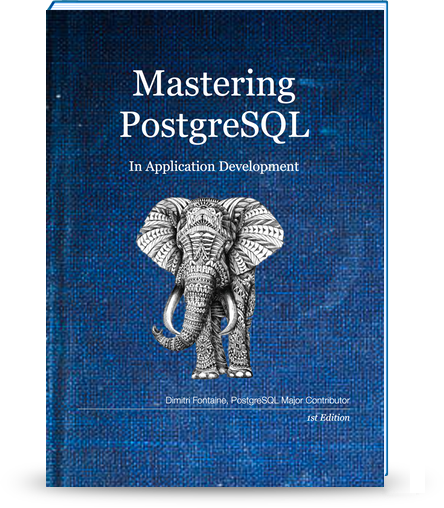
\includegraphics[height=18em]{MasteringPostgreSQLinAppDev-Cover.png}}
    \end{center}
  \end{columns}
\end{frame}

\begin{frame}
  \frametitle{Migrating from another RDBMS to PostgreSQL}

  \begin{center}
    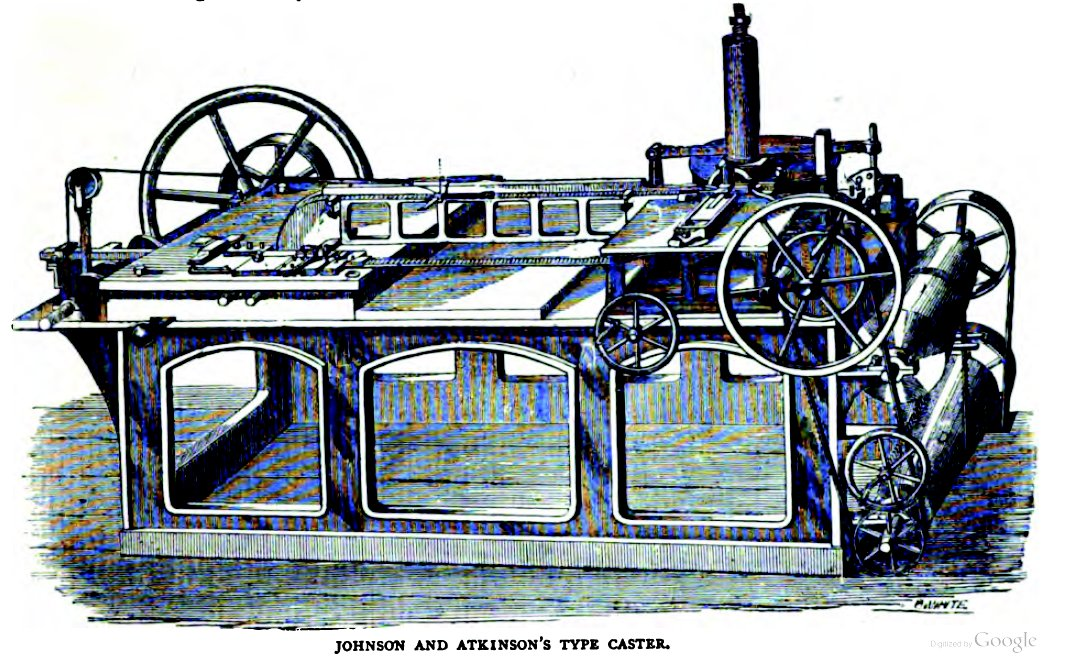
\includegraphics[height=2.1in]{TypeCaster.jpg}
  \end{center}
\end{frame}

\begin{frame}[fragile]
  \frametitle{Why Migrate Over to PostgreSQL?}

  The reasons why migrating are usually a mix of technical choice and budget
  evaluation. Also \textit{human factors}.
  \vfill
  
  \begin{columns}[c]
    \column{.5\textwidth} 
    \begin{center}
      
\includegraphics[height=12em]{cost_effective_black.png}
    \end{center}

    \column{.5\textwidth}
    \begin{itemize}
    \item Cost
    \item Efficiency
    \item Migration Budget, ROI
    \item Expected Behavior (ACID)
    \end{itemize}
  \end{columns}
\end{frame}

{
  \usebackgroundtemplate{
    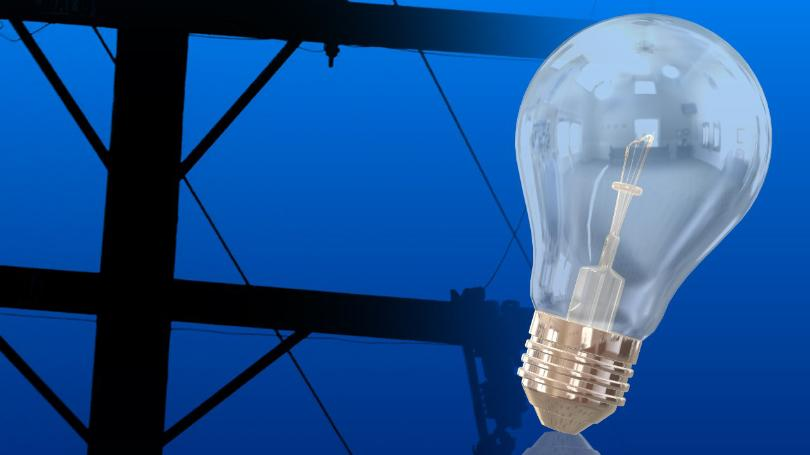
\includegraphics[width=\paperwidth,height=\paperheight]{power-outage.jpg}
  }
  \setbeamercolor{frametitle}{fg=white}
  \begin{frame}
    \setbeamercolor{item}{fg=white}
    \setbeamercolor{normal text}{fg=white}
    \usebeamercolor[fg]{normal text}

    \frametitle{PostgreSQL is fully ACID}

    \texttt{ACID} includes resilience to Power Outages, and a safe and clean
    behavior when used concurrently.
    
    \vfill

    \begin{columns}[c]
      \column{0.3\textwidth} 
      \column{0.7\textwidth}
      \texttt{ACID} stands for:
      \begin{itemize}
      \item Atomic
      \item Consistent
      \item Isolated
      \item \textbf{Durable}
      \end{itemize}
    \end{columns}
  \end{frame}
}

{
  \usebackgroundtemplate {
    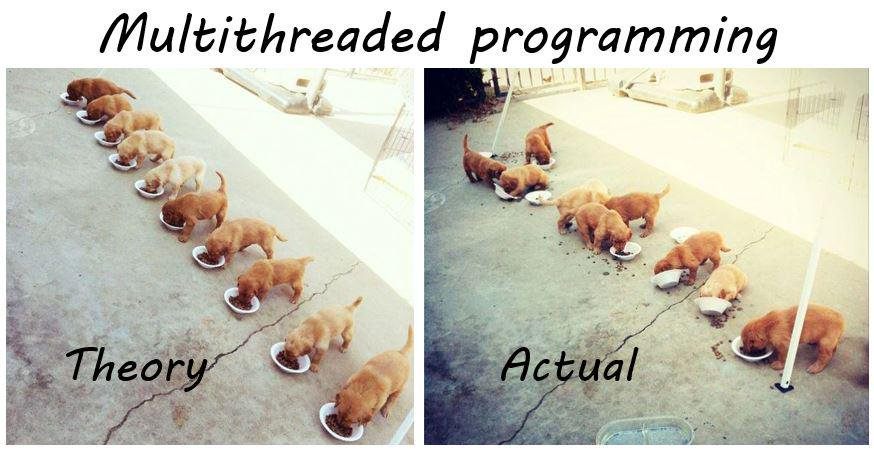
\includegraphics[width=\paperwidth,height=\paperheight]{feeding-puppies.jpg}
  }
  \begin{frame}[plain]
  \end{frame}
}

\begin{frame}[fragile]
  \frametitle{The Migration Project}

  The migration usually isn't done overnight. It requires proper resource
  allocation and planning. And a proper budget, which helps determining the
  return on investment, too.

  \vfill
  
  \begin{columns}[c]
    \column{.5\textwidth} 
    \begin{center}
      
\includegraphics[height=15em]{budget.png}
    \end{center}

    \column{.5\textwidth}
    The migration budget split:
    \begin{itemize}
    \item Data
    \item Code
    \item Service
    \item Opportunity Cost
    \end{itemize}
  \end{columns}
\end{frame}

\section{Difficulties}

{
  \usebackgroundtemplate{
    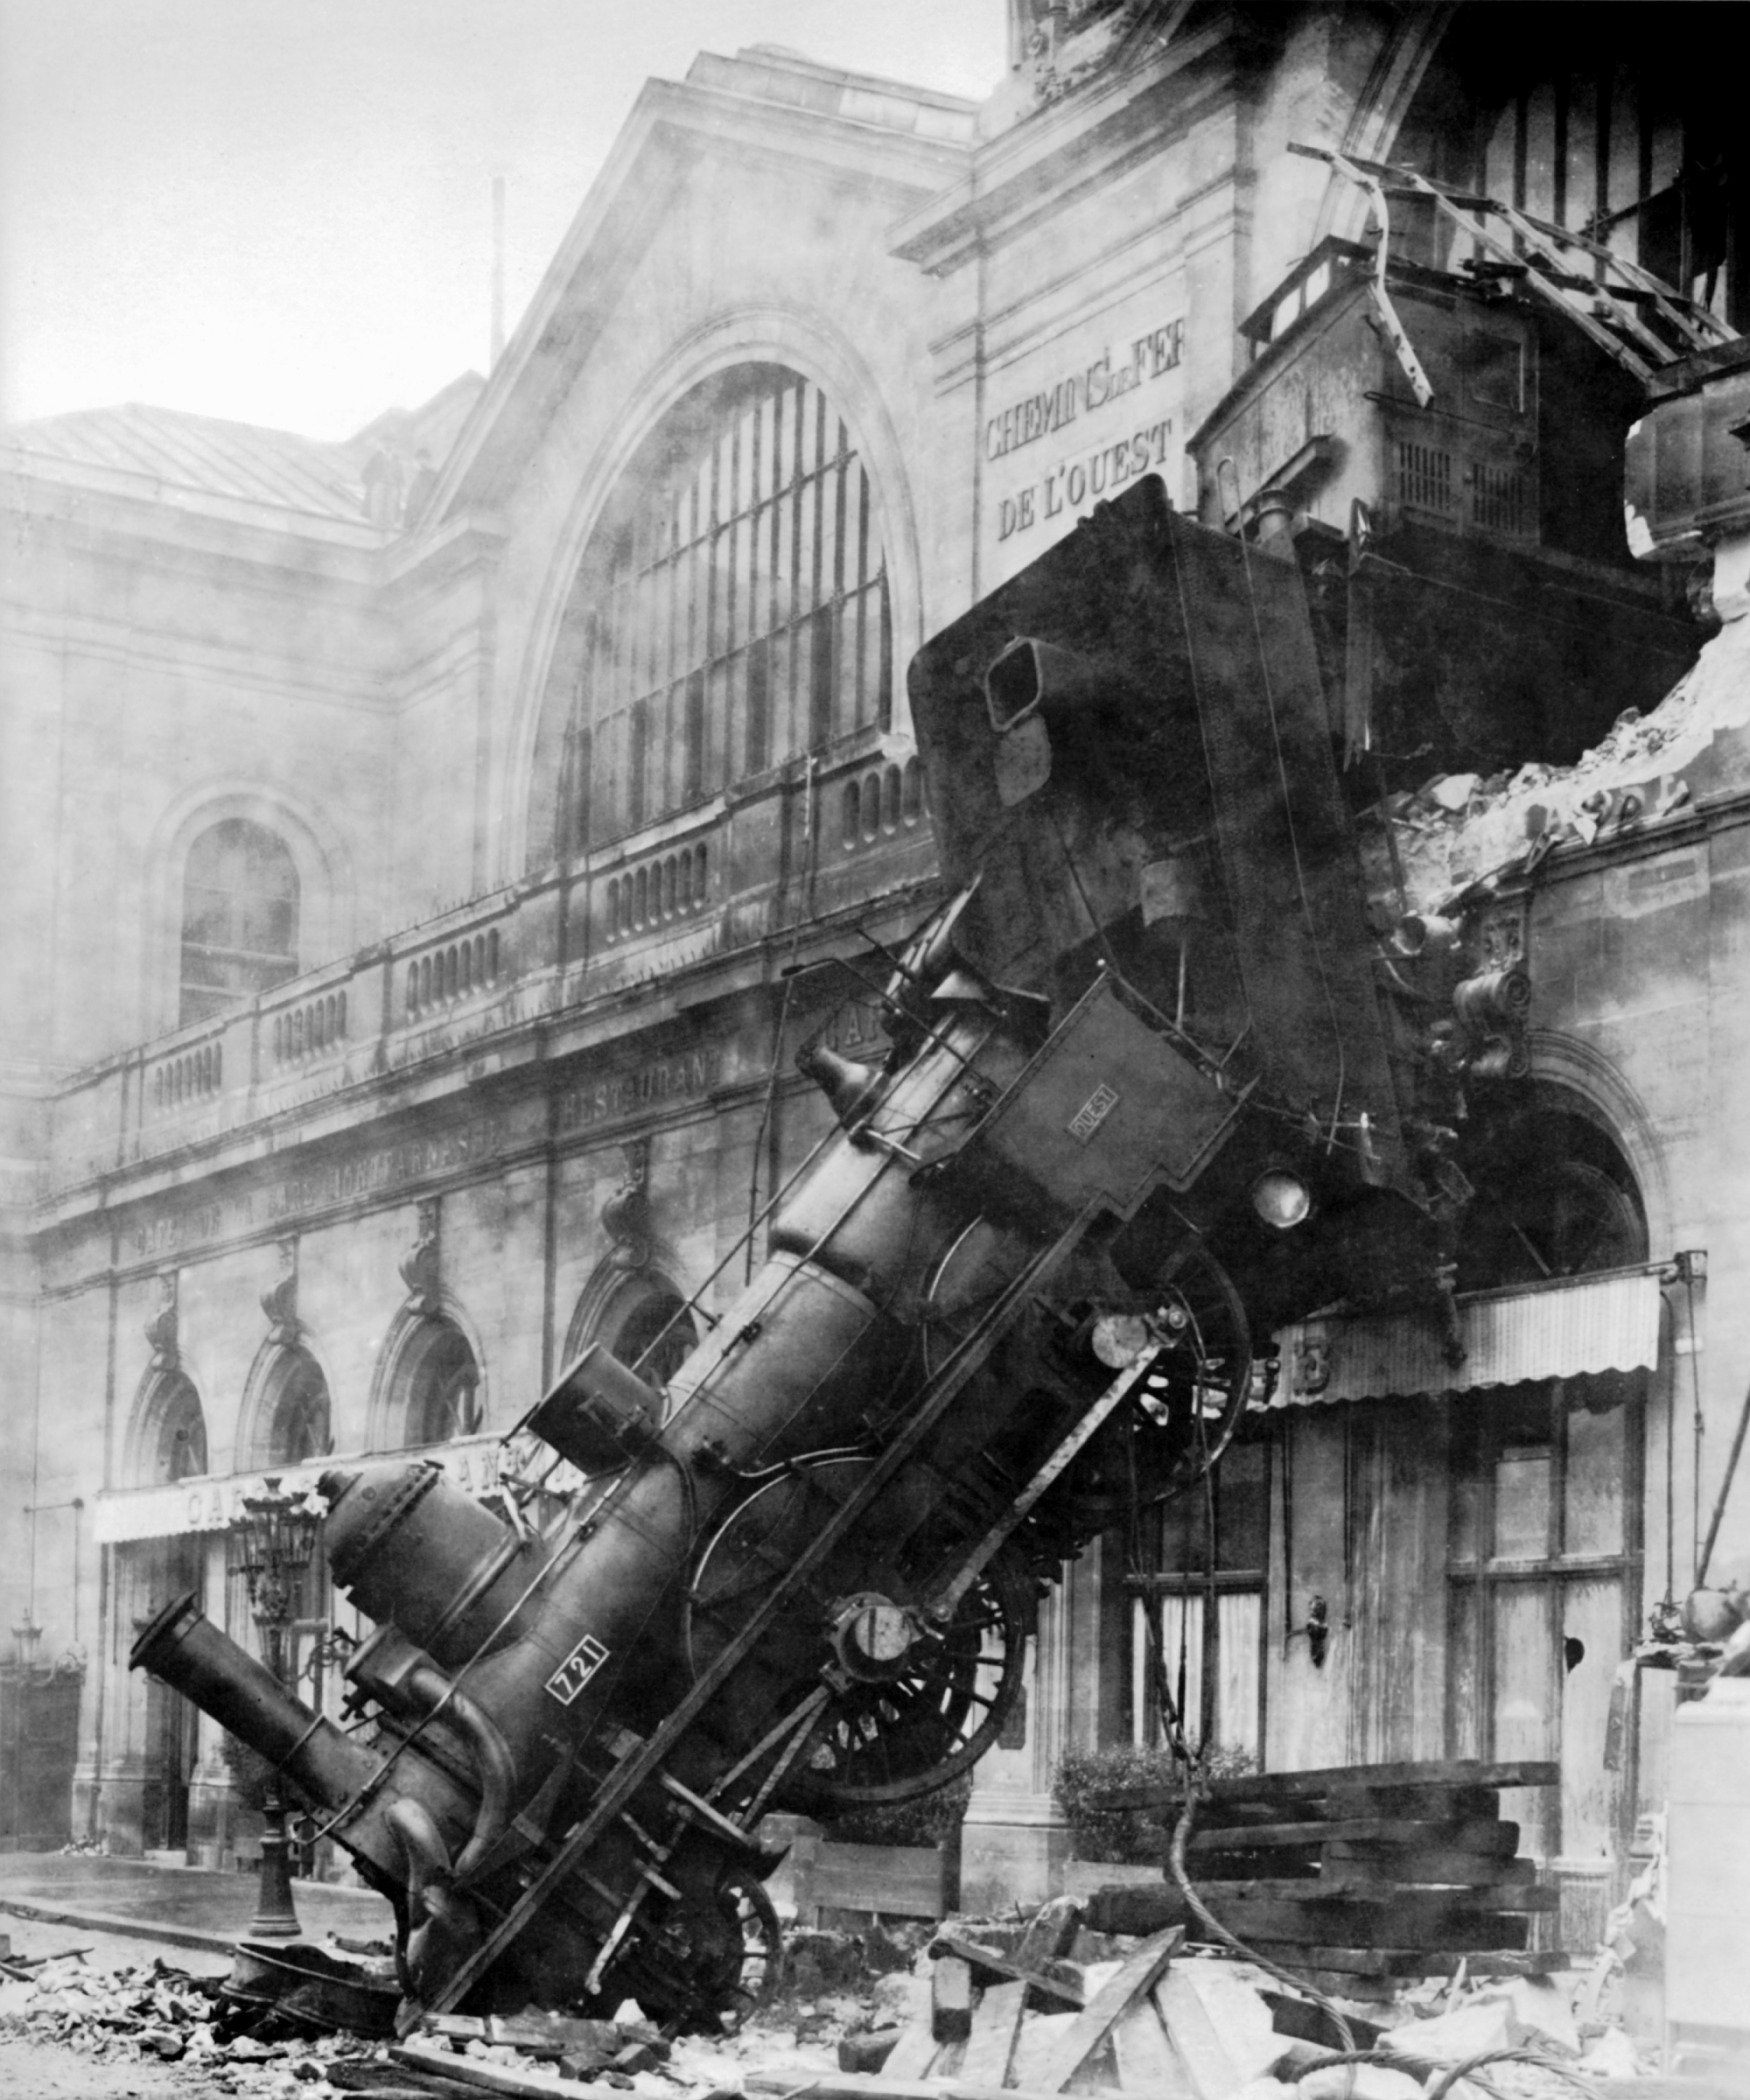
\includegraphics[width=\paperwidth,height=\paperheight]{Train_wreck_at_Montparnasse_1895.jpg}
  }
  \begin{frame}[plain]
    \setbeamercolor{item}{fg=white}
    \setbeamercolor{normal text}{fg=white}
    \usebeamercolor[fg]{normal text}

    \frametitle{Migration Project Planning}

      \begin{flushright}
        \begin{LARGE}
          “A goal without a plan is just a wish”
          \newline
          \newline
          Antoine de Saint-Exupéry
        \end{LARGE}
      \end{flushright}
  \end{frame}
}

\begin{frame}[fragile]
  \frametitle{Migration Planning}

  Migrating the data is often considered a one-off. Then it's not properly
  planned, and happens on the side. Fearing to spend too much time on this,
  proper engineering might not be applied.

  \vfill
  
  \begin{columns}[c]
    \column{.35\textwidth} 
    \begin{center}
      
\includegraphics[height=12em]{round_hole_square_peg_6617.png}
    \end{center}

    \column{.65\textwidth}
    \begin{enumerate}
    \item Setup a PostgreSQL instance
    \item Keep the default configuration
    \item Migrate the data over to PostgreSQL
    \item Manually
    \item In many steps, \textit{error, fix, rinse, repeat}
    \item Including \texttt{\$EDITOR}
    \end{enumerate}
  \end{columns}
\end{frame}

\begin{frame}[fragile]
  \frametitle{Porting the Application}

  Now that we have a PostgreSQL database with the right dataset in there…
  wait, using what schema?

  \vfill
  
  \begin{columns}[c]
    \column{.45\textwidth} 
    \begin{center}
      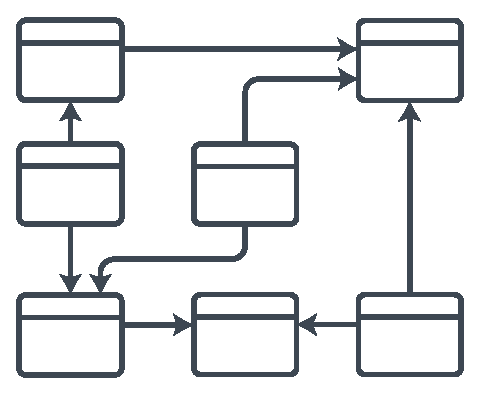
\includegraphics[height=9em]{dbschema.eps}
    \end{center}

    \column{.65\textwidth}
    \begin{itemize}
    \item Same schema, different RDBMS
    \item Sometimes manually converted
    \item Sometimes installed by the ORM
    \item Using only the basics
    \end{itemize}
  \end{columns}
\end{frame}

\begin{frame}[fragile]
  \frametitle{Porting the Application}

  Now that we have a PostgreSQL database with the right dataset in there,
  the code is adjusted until it works as before, only this time using
  PostgreSQL.

  \vfill
  
  \begin{columns}[c]
    \column{.45\textwidth}
    
\includegraphics[height=6em]{editing-your-code.png}

    \column{.65\textwidth}
    Some of the usual traps:
    
    \begin{itemize}
    \item SQL quoting rules
    \item Database Encoding
    \item Client Encoding
    \item SQL syntax
    \end{itemize}
  \end{columns}
\end{frame}

{
  \usebackgroundtemplate {
    
\includegraphics[width=\paperwidth,height=\paperheight]{deploymentplaylist_logo.jpg}
  }
  \begin{frame}[plain]
  \end{frame}
}

\section{A Better Methodology}

{
  \usebackgroundtemplate {
    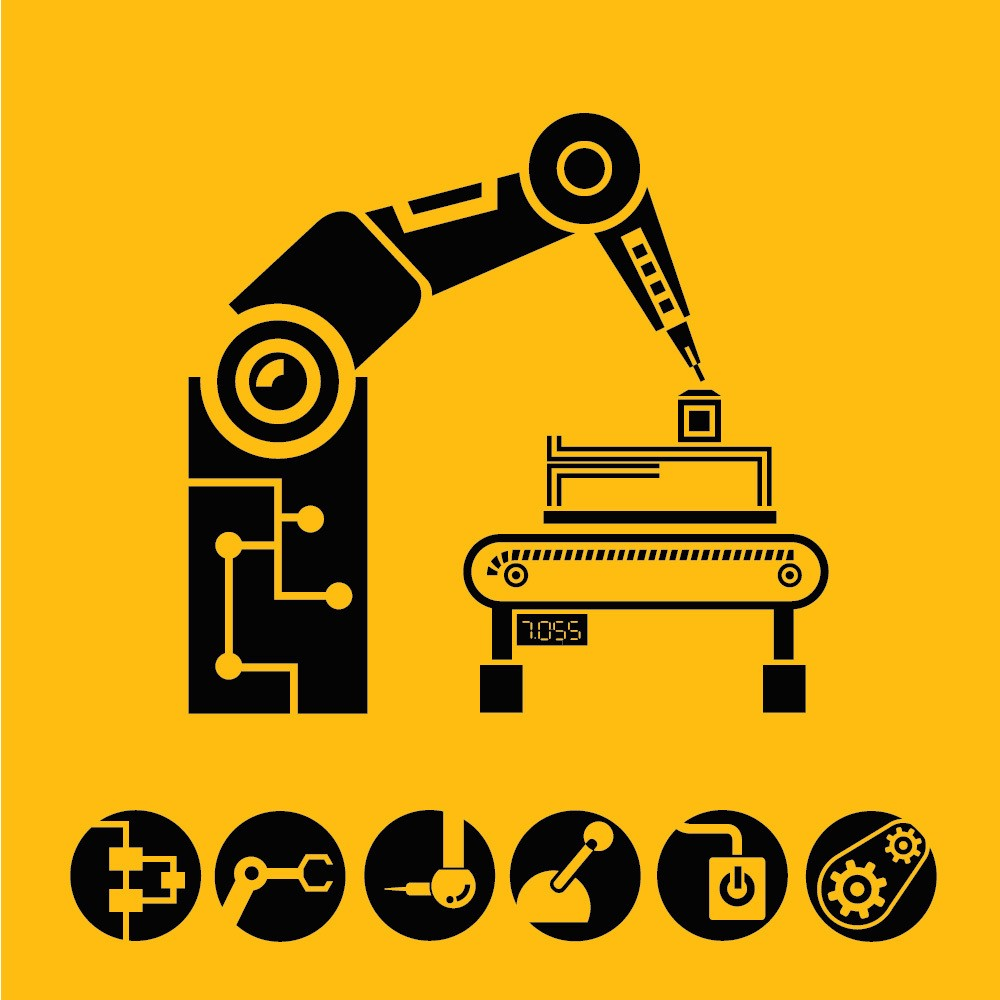
\includegraphics[width=\paperwidth,height=\paperheight]{automate-all-the-things.jpg}
  }
  \begin{frame}[plain]
  \end{frame}
}

\begin{frame}[fragile]
  \frametitle{Continuous Integration, Continuous Delivery}

  \begin{center}
    
\includegraphics[height=18em]{keep-calm-and-automate-all-the-things-13.png}
  \end{center}  
\end{frame}

\begin{frame}[fragile]
  \frametitle{Continuous Integration, Continuous Delivery}

  Instanciate a PostgreSQL version of your application in your
  \textit{CI/CD} setup, from day one, even before doing anything else. Then
  automate all the steps from current production to PostgreSQL based
  production.

  \vfill
  
  \begin{columns}[c]
    \column{.35\textwidth}
    \begin{center}
      
\includegraphics[height=9em]{keep-calm-and-automate-all-the-things-13.png}
    \end{center}

    \column{.75\textwidth}
    From Day One:
    \begin{itemize}
    \item Nightly database migration
    \item All automated, from production data
    \item Add a PostgreSQL coverage dashboard
    \end{itemize}
  \end{columns}
\end{frame}

\section{pgloader}

{
  \usebackgroundtemplate {
    
\includegraphics[width=\paperwidth,height=\paperheight]{howdoidothat.jpg}
  }
  \begin{frame}[plain]
  \end{frame}
}

\begin{frame}[fragile]
  \frametitle{pgLoader loads data into PostgreSQL}

  \center{\url{http://pgloader.io/}}

  \begin{center}
    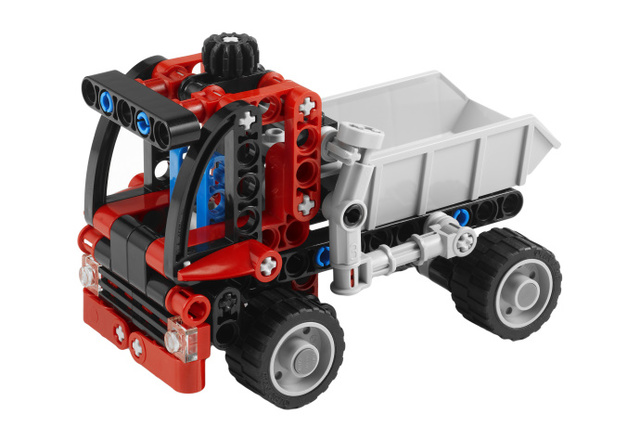
\includegraphics[height=2.1in]{pgloader.jpg}
  \end{center}
\end{frame}

\begin{frame}[fragile]
  \frametitle{pgLoader connects to MySQL}

  \center{\url{http://pgloader.io/howto/mysql.html}}
  \vfill

  \begin{minipage}{0,7\textwidth}
    \begin{minted}[frame=lines,bgcolor=lightgray!30,linenos]{bash}
$ createdb -U user dbname
$ pgloader mysql://user@host/dbname \
           pgsql://user@host/dbname
    \end{minted}
  \end{minipage}

  \begin{center}
    
\includegraphics[height=6em]{mysql.png}
  \end{center}
\end{frame}

\begin{frame}[fragile]
  \frametitle{pgLoader automates all the things}

  When using pgLoader with a \textit{load} command, it's possible to give
  more options:
  
  \vfill
  
  \begin{center}
    \begin{minipage}{0,7\textwidth}
      \begin{minted}
        [frame=lines,bgcolor=beamer@blendedblue!10,linenos]
        {bash}
$ pgloader f1db.load
      \end{minted}
    \end{minipage}
  \end{center}

  \begin{center}
    \begin{minipage}{0,7\textwidth}
      \begin{minted}
        [frame=lines,bgcolor=beamer@blendedblue!10,linenos]
        {sql}
load database
  from mysql://root@localhost/f1db
  into pgsql:///f1db
  with concurrency = 2,
       multiple readers per thread,
       rows per range = 50000
       prefetch rows = 1000000;
      \end{minted}
    \end{minipage}
  \end{center}
\end{frame}

\begin{frame}[plain,fragile]
  \begin{minted}
    [frame=lines,bgcolor=beamer@blendedblue!10,linenos,fontsize=\scriptsize]
    {bash}
               table name     errors       rows      bytes      total time
-------------------------  ---------  ---------  ---------  --------------
          fetch meta data          0         33                     0.325s
           Create Schemas          0          0                     0.001s
         Create SQL Types          0          0                     0.008s
            Create tables          0         26                     0.202s
           Set Table OIDs          0         13                     0.008s
-------------------------  ---------  ---------  ---------  --------------
            f1db.circuits          0         73     8.5 kB          0.039s
  f1db.constructorresults          0      11052   184.6 kB          0.252s
        f1db.constructors          0        208    15.0 kB          0.054s
             f1db.drivers          0        840    79.6 kB          0.094s
            f1db.laptimes          0     417743    10.9 MB          6.320s
                      ...
             f1db.results          0      23597     1.3 MB          0.987s
              f1db.status          0        134     1.7 kB          0.068s
-------------------------  ---------  ---------  ---------  --------------
  COPY Threads Completion          0          4                     6.468s
           Create Indexes          0         20                     2.347s
   Index Build Completion          0         20                     1.458s
          Reset Sequences          0         10                     0.127s
             Primary Keys          0         13                     0.021s
      Create Foreign Keys          0          0                     0.000s
          Create Triggers          0          0                     0.001s
         Install Comments          0          0                     0.000s
-------------------------  ---------  ---------  ---------  --------------
        Total import time          ✓     511270    14.0 MB         10.422s
  \end{minted}
\end{frame}

\begin{frame}[fragile]
  \frametitle{pgLoader example output, 1/3}

  The migration preparation steps: fetch source metadata, apply casting
  rules, transform \textit{default values}, prepare target schema:

  \vfill

  \begin{minted}
    [frame=lines,bgcolor=beamer@blendedblue!10,linenos,fontsize=\small]
    {bash}
               table name       rows      bytes      total time
-------------------------  ---------  ---------  --------------
          fetch meta data         33                     0.325s
           Create Schemas          0                     0.001s
         Create SQL Types          0                     0.008s
            Create tables         26                     0.202s
           Set Table OIDs         13                     0.008s
  \end{minted}
\end{frame}

\begin{frame}[fragile]
  \frametitle{pgLoader example output, 2/3}

  Moving the data over, transforming the data on the fly, and keeping
  batches of rows around in case of \texttt{copy} error(s):
  
  \begin{minted}
    [frame=lines,bgcolor=beamer@blendedblue!10,linenos,fontsize=\small]
    {bash}
               table name        rows      bytes      total time
-------------------------   ---------  ---------  --------------
            f1db.circuits          73     8.5 kB          0.039s
  f1db.constructorresults       11052   184.6 kB          0.252s
        f1db.constructors         208    15.0 kB          0.054s
             f1db.drivers         840    79.6 kB          0.094s
            f1db.laptimes      417743    10.9 MB          6.320s
f1db.constructorstandings       11806   247.3 kB          0.312s
     f1db.driverstandings       31509   714.0 kB          0.971s
            f1db.pitstops        5927   198.7 kB          0.437s
               f1db.races         976    98.4 kB          0.310s
             f1db.seasons          68     3.9 kB          0.395s
          f1db.qualifying        7337   279.0 kB          0.139s
             f1db.results       23597     1.3 MB          0.987s
              f1db.status         134     1.7 kB          0.068s
  \end{minted}
\end{frame}

\begin{frame}[fragile]
  \frametitle{pgLoader example output, 3/3}

  Now that the data has been migrated over, complete the PostgreSQL schema
  with \textit{Primary Keys}, \textit{Foreign Keys}, \textit{Sequences},
  etc:
  \vfill
  
  \begin{minted}
    [frame=lines,bgcolor=beamer@blendedblue!10,linenos,fontsize=\small]
    {bash}
               table name        rows      bytes      total time
-------------------------    ---------  ---------  --------------
  COPY Threads Completion            4                     6.468s
           Create Indexes           20                     2.347s
   Index Build Completion           20                     1.458s
          Reset Sequences           10                     0.127s
             Primary Keys           13                     0.021s
      Create Foreign Keys            0                     0.000s
          Create Triggers            0                     0.001s
         Install Comments            0                     0.000s
-------------------------    ---------  ---------  --------------
        Total import time       511270    14.0 MB         10.422s
  \end{minted}
\end{frame}

{
  \usebackgroundtemplate {
    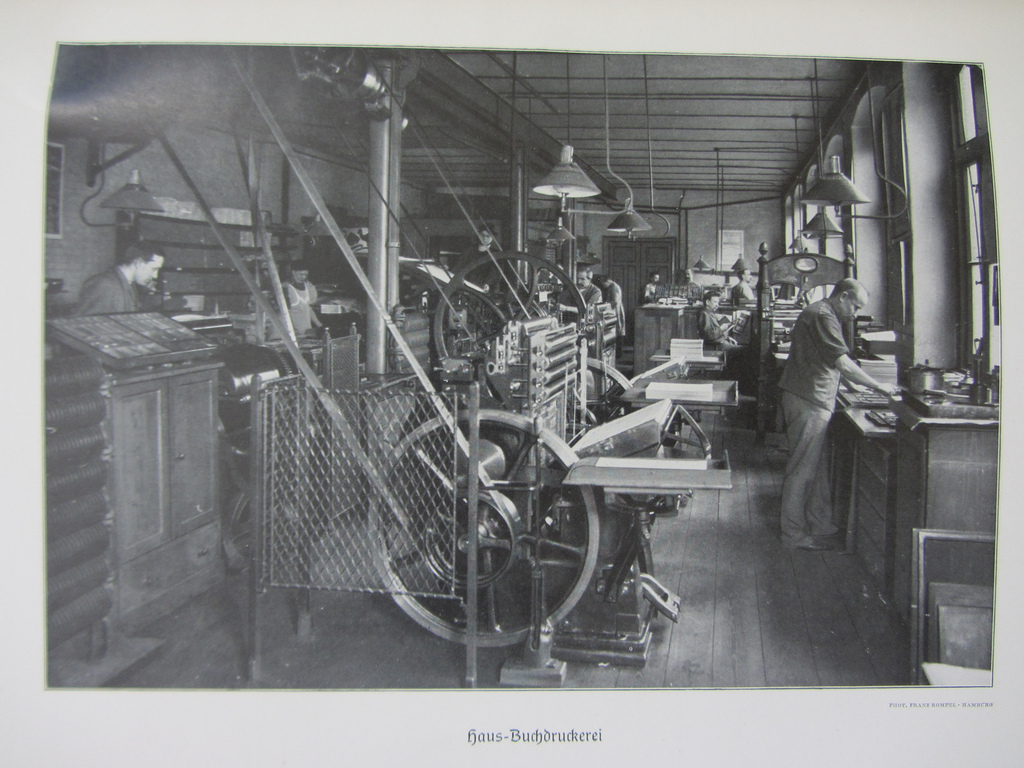
\includegraphics[width=\paperwidth,height=\paperheight]{Haus-Type-Caster.jpg}
  }
  \begin{frame}[plain]
  \end{frame}
}

\begin{frame}[fragile]
  \frametitle{pgLoader Casting Rules}

  In order to be fully automated, pgloader allows its users to redefine any
  default casting rule.
  \vfill

  \begin{minted}
    [frame=lines,bgcolor=beamer@blendedblue!10,linenos]
    {plpgsql}
load database
     from mysql://root@unix:/tmp/mysql.sock:3306/pgloader
     into postgresql://dim@localhost/pgloader

 alter schema 'pgloader' rename to 'mysql'

 CAST column base64.id to uuid drop typemod drop not null,
      column base64.data to jsonb using base64-decode,

      type decimal when (and (= 18 precision) (= 6 scale))
        to "double precision" drop typemod

 before load do $$ create schema if not exists mysql; $$;
  \end{minted}
\end{frame}

\begin{frame}[fragile]
  \frametitle{pgLoader Catalog Mapping}

  pgloader maintains an internal representation of both the \textit{source}
  and \textit{target} catalogs, allowing to apply some internal commands in
  order to implement the mapping:

  \vfill
  
  \begin{columns}[c]
    \column{.45\textwidth}
    \begin{center}
      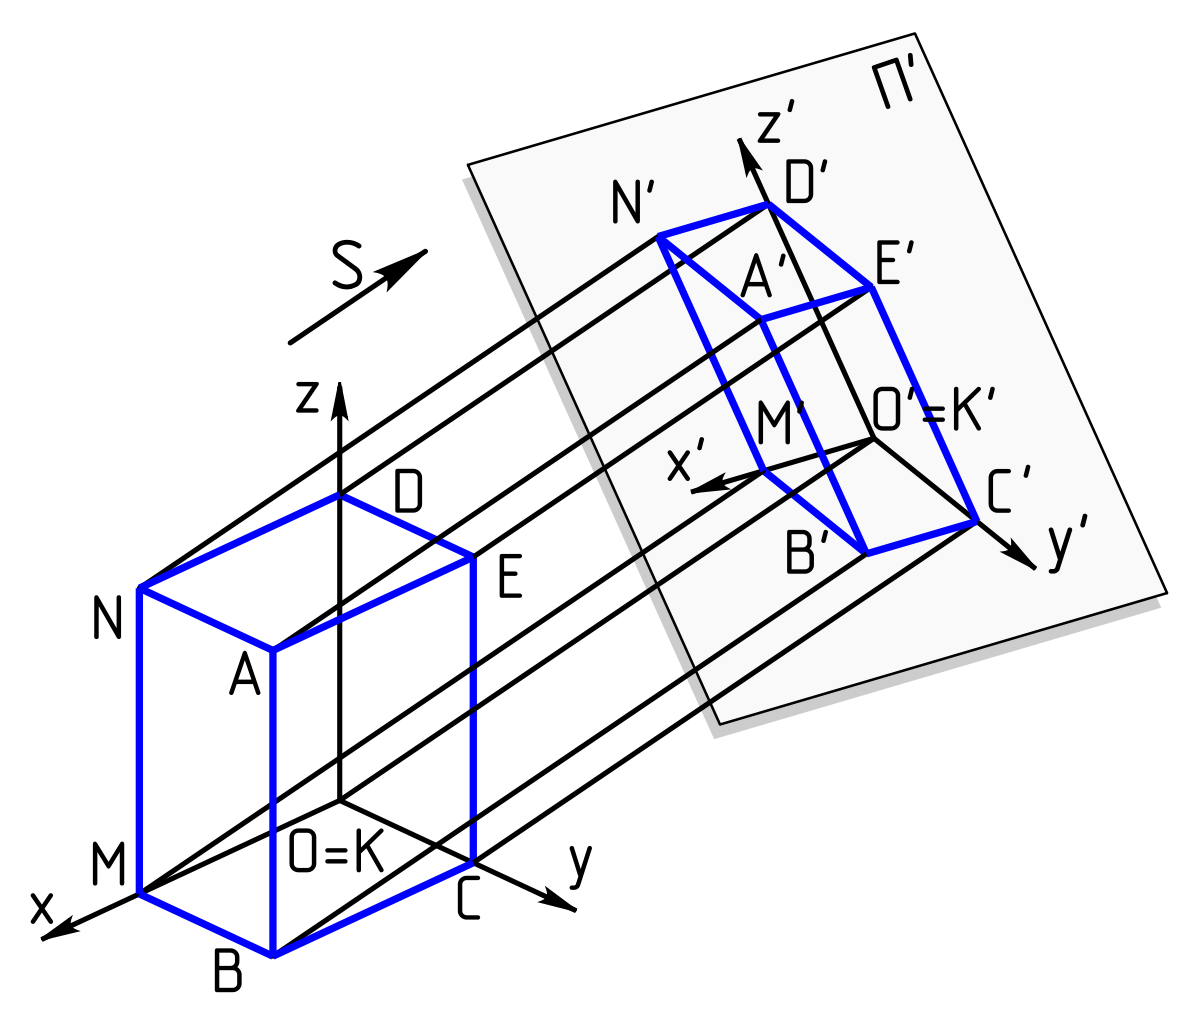
\includegraphics[height=12em]{Axonometric_projection.png}
    \end{center}

    \column{.65\textwidth}
    \begin{center}
      \begin{minipage}{0,8\textwidth}
        \begin{minted}[frame=lines,bgcolor=beamer@blendedblue!10,linenos]{sql}
ALTER SCHEMA '...'
      RENAME TO '...'

ALTER TABLE NAMES MATCHING ...
      IN SCHEMA '...'

ALTER TABLE NAMES MATCHING ...
      RENAME TO '...'
        \end{minted}
      \end{minipage}
    \end{center}
  \end{columns}
\end{frame}

{
  \usebackgroundtemplate{    
    \begin{tikzpicture}[remember picture,overlay]
      \node[opacity=0.45] at (current page.center) {
        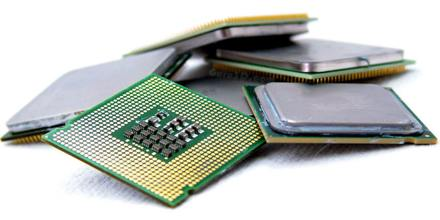
\includegraphics{Multi-Core-Processor00.jpg}
      };
    \end{tikzpicture}
  }

  \begin{frame}[fragile]
    \frametitle{pgLoader Parallelism and Concurrency}

    Multiple operations are done in parallel in pgloader, in order to
    improve pgloader efficiency. Several parameters allow to control its
    parallel behavior.

    \vfill
    
    \begin{columns}[c]
      \column{0.3\textwidth} 
      \column{0.7\textwidth}
      Parallel Operations cover:
      \begin{itemize}
      \item Reader/Writer
      \item \texttt{CREATE INDEX}
      \item Including \textsc{Primary Keys!}
      \item Multiple tables
      \item Same table with a key range
      \end{itemize}

    \end{columns}  
  \end{frame}
}

\begin{frame}[fragile]
  \frametitle{pgLoader Materialize Views}

  Rather than copying plain table from MySQL to PostgreSQL, it is possible
  to copy the result of \texttt{SELECT * FROM view;} instead.
  
  \begin{center}
    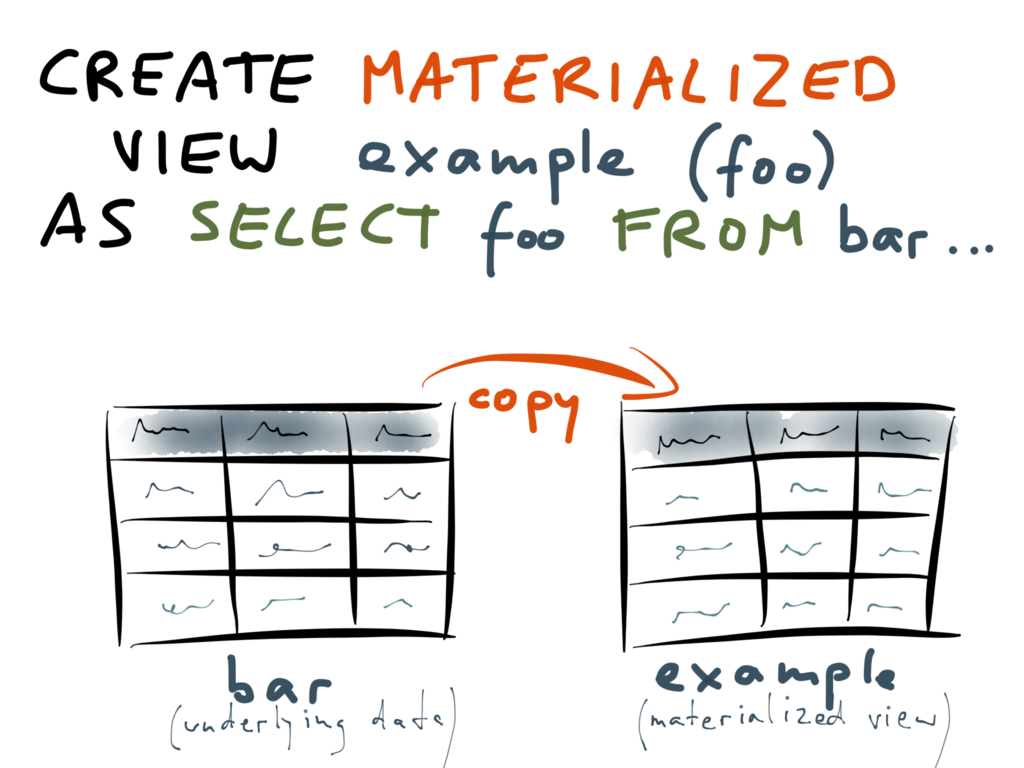
\includegraphics[height=18em]{slide-22.png}
  \end{center}
\end{frame}

\begin{frame}[fragile]
  \frametitle{Other pgLoader Options}

  Taken from several test files, a \textit{hodgepodge}:
  
  \begin{minted}
    [frame=lines,bgcolor=beamer@blendedblue!10,linenos,fontsize=\small]
    {plpgsql}
load database
     from '{{DBPATH}}'
     into postgresql:///pgloader
    
 WITH on error stop, concurrency = 2, workers = 6,
      prefetch rows = 25000, rows per range = 50000,
      multiple readers per thread,
      max parallel create index = 4,
      quote identifiers

  SET PostgreSQL PARAMETERS
      maintenance_work_mem to '128MB', work_mem to '12MB',
      search_path to 'sakila, public, "$user"'

  SET MySQL PARAMETERS
      net_read_timeout  = '120', net_write_timeout = '120'  
    \end{minted}
\end{frame}

\begin{frame}[fragile]
  \frametitle{Other pgLoader Options}

  Taken from the \texttt{test/sakila.load} file:
  
  \begin{minted}
    [frame=lines,bgcolor=beamer@blendedblue!10,linenos,fontsize=\small]
    {plpgsql}
   BEFORE LOAD
     DO
       $$ create extension if not exists ip4r; $$,
       $$ create schema if not exists geolite; $$

     EXECUTE 'geolite.sql'

   -- WITH create no tables, include drop, truncate,
           
   --      include drop, create tables, no truncate,
   --      create indexes, reset sequences, foreign keys
     
   INCLUDING ONLY TABLE NAMES MATCHING ~/film/, 'actor'
   EXCLUDING TABLE NAMES MATCHING ~<ory>

    \end{minted}
\end{frame}

\begin{frame}[fragile]
  \frametitle{pgLoader Data Sources}

  \begin{columns}[c]
    \column{.5\textwidth} 
    \begin{center}
      
\includegraphics[height=6em]{dBase.png}
    \end{center}
    \column{.5\textwidth}
    \begin{center}
      
\includegraphics[height=6em]{SQLite.png}
    \end{center}
  \end{columns}
  
  \begin{columns}[c]
    \column{.5\textwidth}
    \begin{center}
      
\includegraphics[height=6em]{mysql.png}
    \end{center}
    \column{.5\textwidth}
    \begin{center}
      
\includegraphics[height=6em]{mssql.png}
    \end{center}
  \end{columns}
\end{frame}

\section{User Testimonials}

{
  \usebackgroundtemplate{
    
\includegraphics[width=\paperwidth,height=\paperheight]{Rating.jpg}
  }
  \setbeamercolor{frametitle}{fg=white}
  \begin{frame}[plain]
    \frametitle{Some User Testimonials}
  \end{frame}
}

{
  \usebackgroundtemplate{
    \begin{tikzpicture}[remember picture,overlay]
      \node[opacity=0.4] at (current page.center) {
        
\includegraphics {twitter-logo.png}
      };
    \end{tikzpicture}
  }

  \begin{frame}[fragile]
    \frametitle{Feedback from Twitter}

    \begin{center}
      \begin{minipage}{0,6\textwidth}
        \begin{minipage}{0,2\textwidth}
          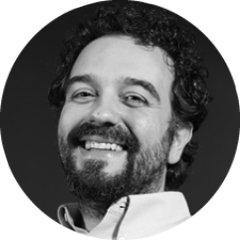
\includegraphics[height=3em]{tommasomatic.png}
        \end{minipage}
        \begin{minipage}{0,8\textwidth}
          Tommaso Patrizi \newline
          \texttt{@tommasomatic}
        \end{minipage}
      \end{minipage}
      \rule[10pt]{0,6\textwidth}{1px}
      
      \begin{minipage}{0,6\textwidth}
        \begin{Large}
          @tapoueh \#pgloader is so good I'm almost crying! Say goodbye to
          all mysql implementations! Thanks!
        \end{Large}
      \end{minipage}
      \rule{0,6\textwidth}{1px}

      \vfill
      \url{https://twitter.com/tommasomatic/status/884181490724155392}
    \end{center}
  \end{frame}
}

{
  \usebackgroundtemplate{
    \begin{tikzpicture}[remember picture,overlay]
      \node[opacity=0.4] at (current page.center) {
        
\includegraphics {twitter-logo.png}
      };
    \end{tikzpicture}
  }

  \begin{frame}[fragile]
    \frametitle{Feedback from Twitter}

    \begin{center}
      \begin{minipage}{0,6\textwidth}
        \begin{minipage}{0,2\textwidth}
          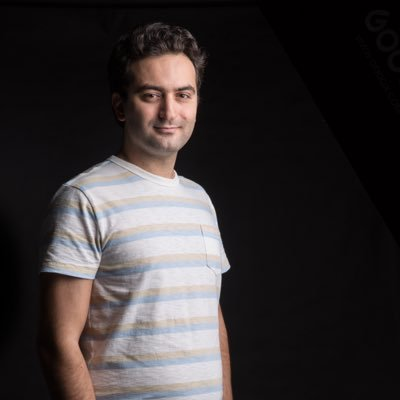
\includegraphics[height=3em]{majid_hajian.jpg}
        \end{minipage}
        \begin{minipage}{0,8\textwidth}
          Majid Hajian \newline
          \texttt{@mhadaily}
        \end{minipage}
      \end{minipage}
      \rule[10pt]{0,6\textwidth}{1px}
      
      \begin{minipage}{0,6\textwidth}
        \begin{Large}
          Successfully migrated from \#MySQL 5 to \#PostgreSQL 9.5, roughly
          16GB data, thanks to \@tapoueh for a fantastic \#pgloader tool
        \end{Large}
      \end{minipage}
      \rule{0,6\textwidth}{1px}

      \vfill
      \url{https://twitter.com/mhadaily/status/806763214092414976}
    \end{center}
    
  \end{frame}
}

{
  \usebackgroundtemplate{
    \begin{tikzpicture}[remember picture,overlay]
      \node[opacity=0.4] at (current page.center) {
        
\includegraphics {twitter-logo.png}
      };
    \end{tikzpicture}
  }

  \begin{frame}[fragile]
    \frametitle{Feedback from Twitter}

    \begin{center}
      \begin{minipage}{0,6\textwidth}
        \begin{minipage}{0,2\textwidth}
          
\includegraphics[height=3em]{whitequark.png}
        \end{minipage}
        \begin{minipage}{0,8\textwidth}
          whitequark \newline
          \texttt{@whitequark}
        \end{minipage}
      \end{minipage}
      \rule[10pt]{0,6\textwidth}{1px}
      
      \begin{minipage}{0,6\textwidth}
        \begin{Large}
          so I need to migrate $\sim$17 million rows from MySQL to Postgres.
          am I in for pain or for a lot of pain?
        \end{Large}
      \end{minipage}
      \rule[10pt]{0,6\textwidth}{1px}

      \begin{minipage}{0,6\textwidth}
        \begin{Large}
          pgloader appears to be able to do it in $\sim$1 hour, with 512MB
          of RAM (probably faster with more RAM)
        \end{Large}
      \end{minipage}
      \rule{0,6\textwidth}{1px}

      \vfill
      \url{https://twitter.com/whitequark/status/768208585503354881}
    \end{center}
    
  \end{frame}
}

\section{Contributing}

{
  \usebackgroundtemplate{
    
\includegraphics[width=\paperwidth,height=\paperheight]{participation-cc.png}
  }
  \begin{frame}[plain]
  \end{frame}
}

\begin{frame}
  \frametitle{pgloader: Open Source, github}

  \center{\url{https://github.com/dimitri/pgloader}}

  \begin{center}
    
\includegraphics[height=2.1in]{Octocat.png}
  \end{center}
\end{frame}

\begin{frame}[fragile]
  \frametitle{Contributing to pgLoader}

  Maintaining pgloader is fun: you get to help automate advanced PostgreSQL
  migrations, from diverse environments. Common Lisp is easy enough to
  learn, of course new APIs and ecosystems are not always easy to grasp.
  
  \begin{columns}[c]
    \column{.4\textwidth}
    \begin{center}
      
\includegraphics[height=12em]{lisplogo_warning2_256.png}
    \end{center}

    \column{.6\textwidth}
    Ideas of areas where to contribute:
      \begin{itemize}
      \item Windows™ Automatic Builds
      \item Keep Build Artefacts from Travis
      \item More tests coverage
      \item Documentation: tutorials
      \item From issues to the wiki
      \item Other Feature Requests
    \end{itemize}
  \end{columns}  
\end{frame}

{
  \usebackgroundtemplate{
    \tikz\node[opacity=0.6] {
      
\includegraphics[width=\paperwidth,height=\paperheight]{piggy.png}
    };
  }
  \begin{frame}
    \frametitle{The pgLoader Moral Licence}

    \begin{Large}
      \begin{center}
        To contribute financially to the project, buy a
        \vfill
        pgloader Moral Licence
        \vfill
        \url{http://pgloader.io/pgloader-moral-license.html}
      \end{center}
    \end{Large}
    \vfill
  \end{frame}
}

{
  \usebackgroundtemplate{
    \begin{tikzpicture}[remember picture,overlay]
      \node[opacity=0.4] at (current page.center) {
        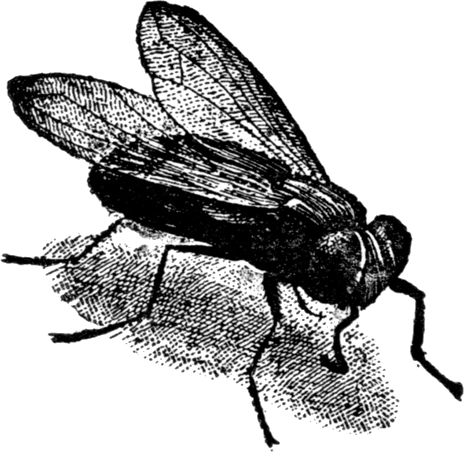
\includegraphics[width=0.8\paperwidth,height=0.8\paperheight]{fly.png}
      };
    \end{tikzpicture}
  }
 
  \begin{frame}
    \frametitle{Questions?}

    \begin{center}
      \textbf{\Large Now is the time to ask!}
    \end{center}
  \end{frame}
}

\end{document}
